\documentclass{article}
\usepackage{amsmath}
\usepackage{amssymb}
\usepackage{graphicx}

    
\begin{document}
\section*{Question 1}
The matroid has no parallel pairs, so the only cycles are of length 3+. The graph will have 
9 edges, and  a spanning tree will be of size 4. As seen in class, we can assume the graph is connected, and so there are 4+1=5 vertices,
due to the fact that in a connected graph with $n$ vertices, there are $n-1$ edges in a spanning tree.
I began by listing all 3-cycles.

If edges are in a 3 cycle, they must share a vertex. Thus, $a$ shares vertices with $b, d, c, e$. We see that $d, e$ share a vertex, and as they both 
share a vertex with a, we know all 3 edges meet at the same point. This, together with the 3 cycles, determines the positions of $a, b, c, d, e, f$.
At this stage, we have one vertex without any edges. We know $g, d, h$ is a circuit, and all edge spots apart from the two between $d$ and this empty 
vertex are full. Hence $g, h$ must take these edges. Additionally, $h, f, i$ is a circuit, and so $h$ must also share a vertex with $f$. This determines 
the location of $g, h$, and therefore $i$. 

It is simple to verify that this graph generates the above matroid.

    \begin{figure}[!htb]
        \centering
        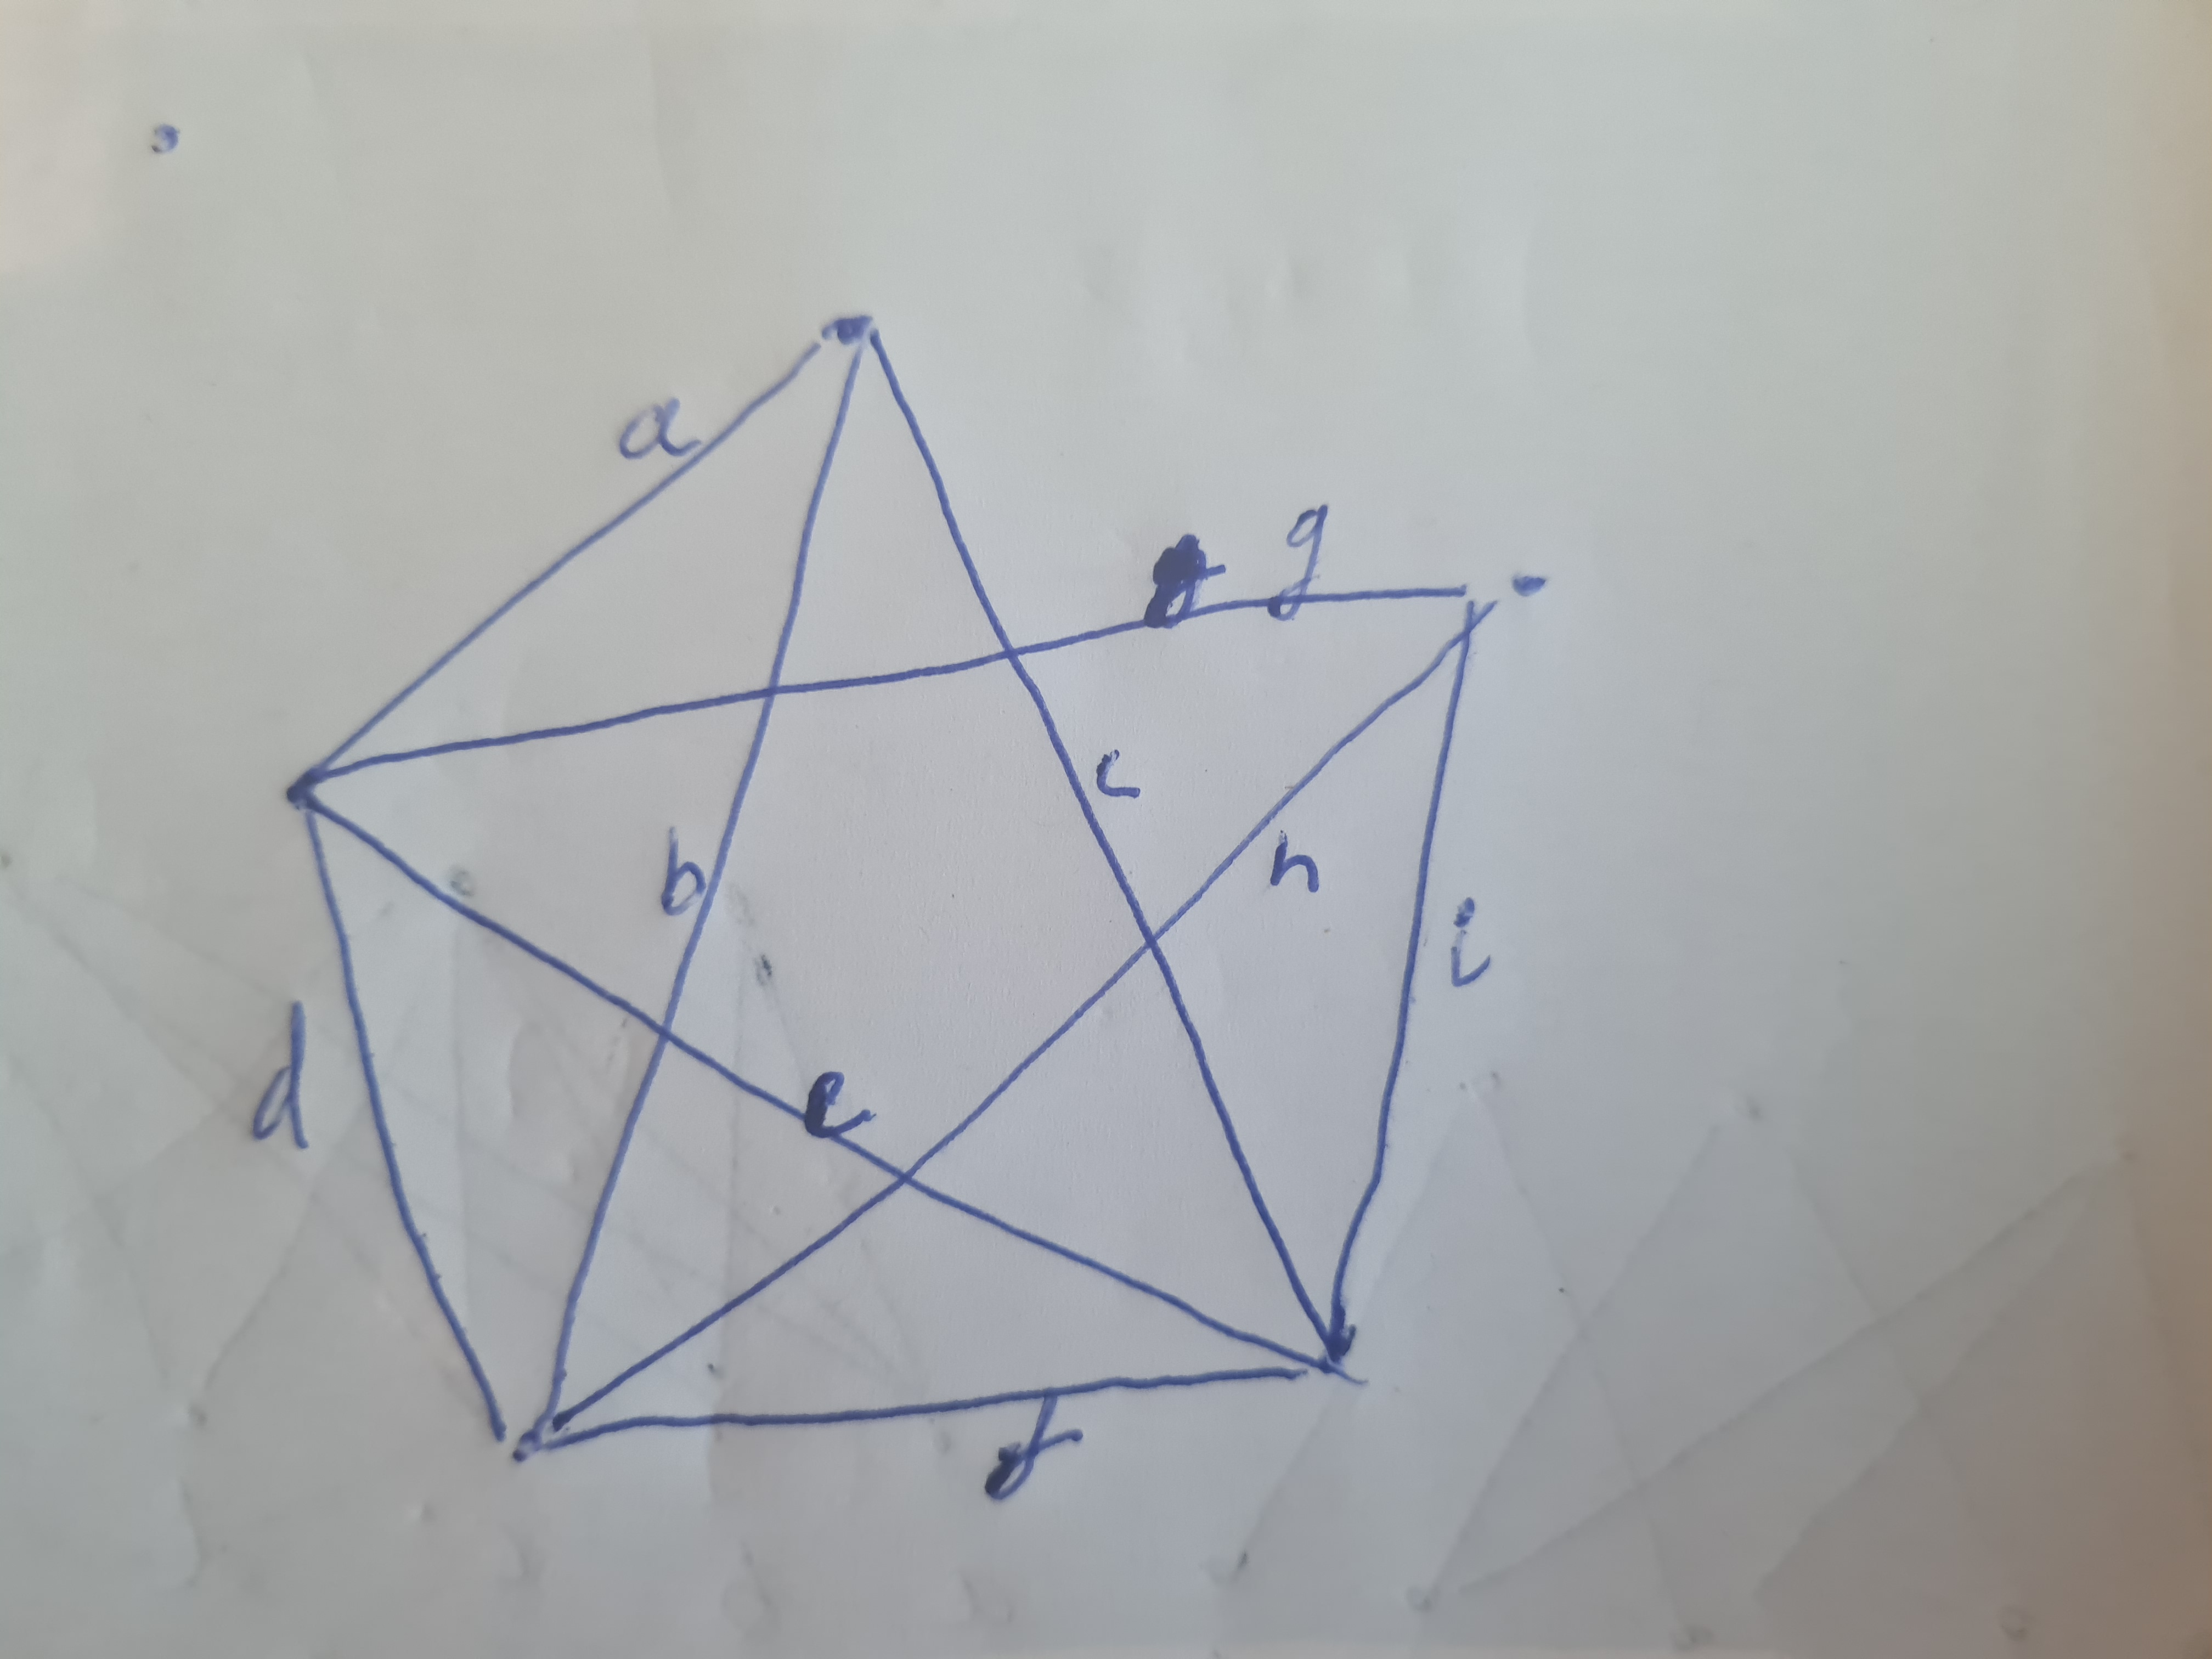
\includegraphics[width=0.5\textwidth]{q1.jpg}
        \caption{Question 1}
    \end{figure}

\section*{Question 2}
We can immediately see that $\{a, c, d, h\}$ is a 4-element independent set. The geometric presentation is in $\mathbb{R}^3$, so 
we will set these 4 elements to be the identity vectors $I_4$.

Now, observe that if 4 elements are coplaner (in this case, therefore a circuit), then none of their coefficients can be 0 in a linear sum,
as 3 coplanar elements (that are not colinear) are linearly independent.
If one was, then we would have a dependent subset of size 3, for a contradiction. Thus over $GF(2)$, their coefficients must all be 1.
So, at this point, we see that $\{a, c, d, g\}$ is a circuit, and only $g$ is undefined. This allows us to solve for $g$'s vector.
The same is done for $e$ via $\{a, e, h, d\}$, $b$ via $\{b, e, g, d\}$, and finally $f$ via $\{d, f, h, g\}$.

A simple check verifies that this is indeed a vector representation of the matroid.

\[
    \bordermatrix{
        & a & c & d & h & b & e & f & g \cr
        & 1 & 0 & 0 & 0 & 0 & 1 & 1 & 1 \cr
        & 0 & 1 & 0 & 0 & 1 & 0 & 1 & 1 \cr
        & 0 & 0 & 1 & 0 & 1 & 1 & 0 & 1 \cr
        & 0 & 0 & 0 & 1 & 1 & 1 & 1 & 0
            }
\]
\section*{Question 3}
Immediately it is clear that $a, b, c$ are independent. Our bases are of size 3, so our geometric representation will be in $\mathbb{R}^2$.
Firstly, note that any 3-element subset of $\{a, h, f, g\}$
is linearly dependent. This can only happen should all 4
elements be colinear.

Now $\{a, b, d\}$ is dependent, as is $\{b, c, f\}$ and $\{a, c, e\}$.
So, a and b must be connected by a line (via d), as must a and c (via e). Finally, the line through b and c
must pass through f. Hence we try a triangle around the 4 colinear points (and hope that works).

Now that the position is relatively fixed, the rest is easy. 
We see $\{b, g, e\}$ is colinear, as are $\{c, d, g\}$.
We also have $e+h+d=0$, so these are colinear also.

Now $b$ is connected to a, g, and f, and it cannot be connected to $h$,
as $b+h=(1, 0, 2)$, which no other vector is equipped to deal with.
A similar story is true for $c$ and $h$.

At this point we are done!



\begin{figure}[!htb]
    \centering
    \includegraphics[width=0.5\textwidth]{q3.jpg}
    \caption{Question 3}
\end{figure}

\section*{Question 4}
It's actually easier to construct a matroid that is not transversal, and then show that its dual is indeed transversal.
Consider the following geometric presentation of a rank 2 matroid.
\begin{figure}[!htb]
    \centering
    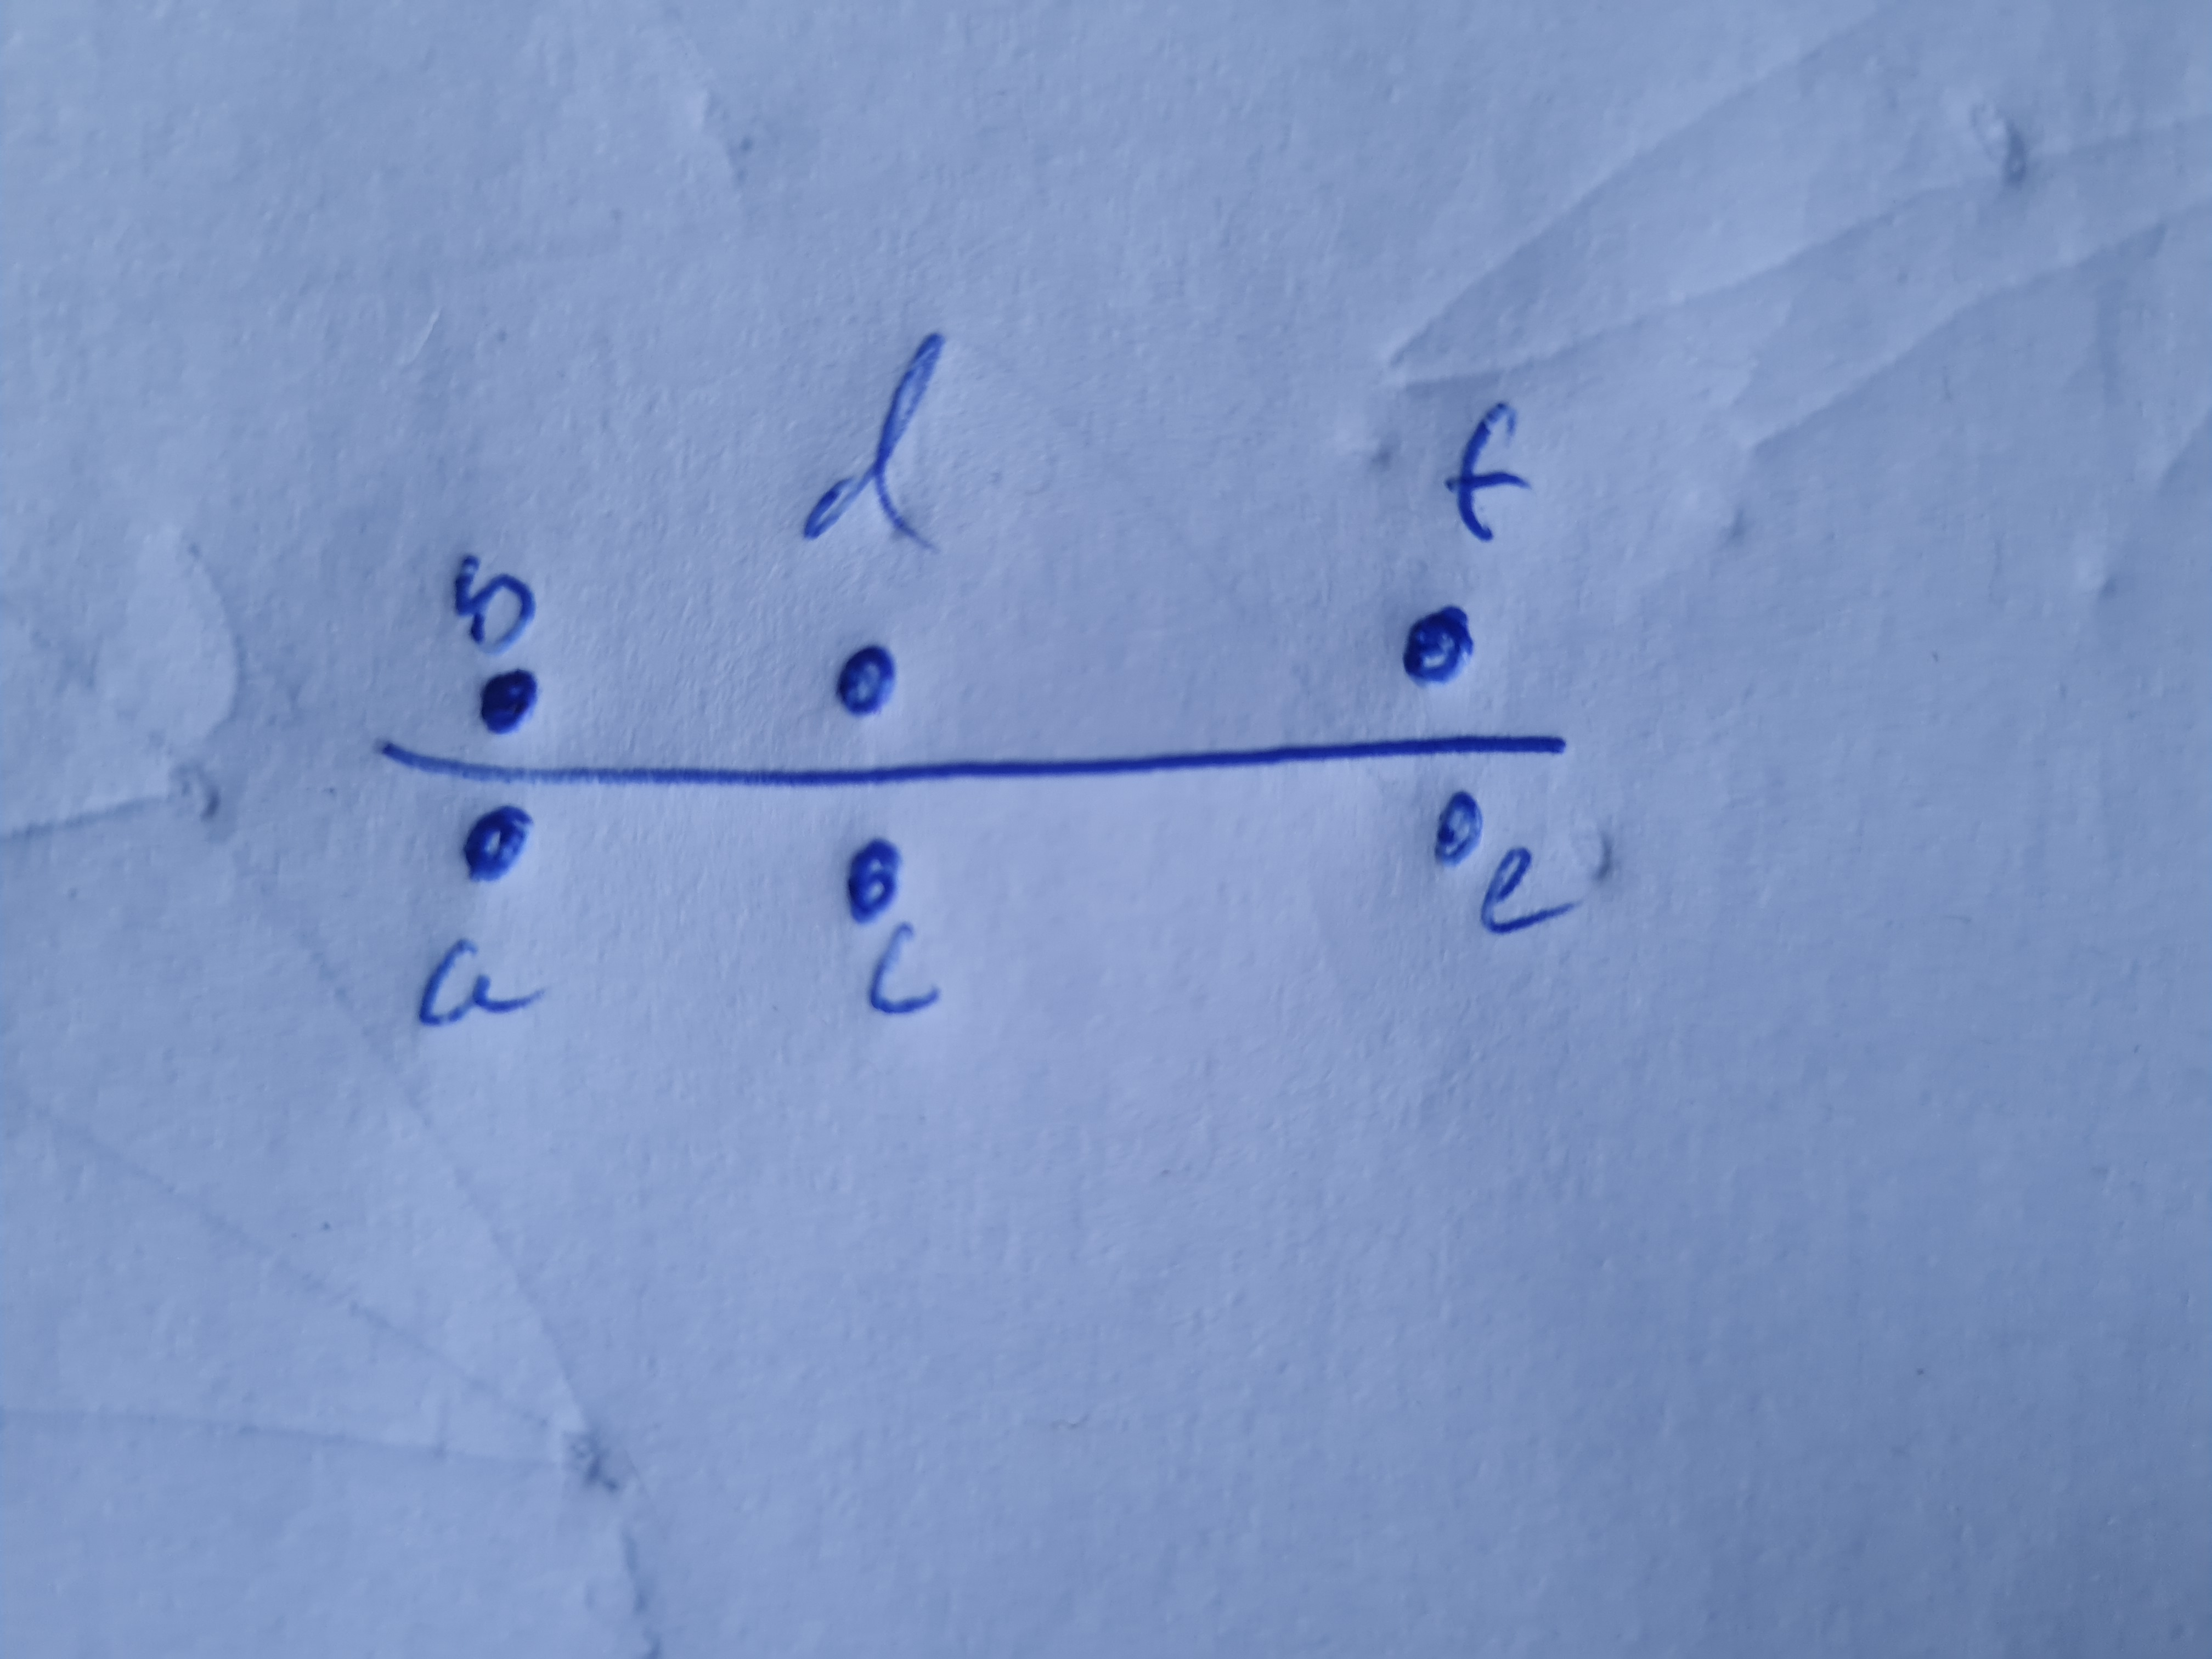
\includegraphics[width=0.5\textwidth]{q4main.jpg}
    \caption{Geometric representation of a nontransversal matroid}
\end{figure}

We claim this matroid is not transversal, but its dual is.
Firstly, that $M$ is not transversal. Now, suppose that there are more than 2 vertices on the side we are matching to
(I.e. the side whose vertex set is not $\{a, b, c, d, e, f\}$). Every vertex can form a basis, so is matchable.
Each of $\{a, b\}$, $\{c, d\}$, $\{e, f\}$ are parallel pairs and so cannot form a basis. This means each such pair must map to the same vertex! (if 
they didn't we could create a basis of size 2). Now if we had 3 or more vertices on the matching side, then in any non-trivial use of those vertices,
we could create a matchable set of size 3 or more, for a contradiction to the fact that $M$ has rank 2.
For example, say $\{a, b\}$ both connect to vertex 1, and $\{c, d\}$ to vertex 2. Any vertex mapping to 3 therefore allows us to make a basis of size 3.
However, if we had only 2 vertices, then $\{a, b\}$ maps somewhere, w.l.o.g. to vertex 1. $\{a, c\}$ is a basis, and so $c$ (and therefore $d$) both map to vertex 2.
However, so do $\{a, e\}$, and thus $e, f$ must both match to vertex 2 as well (see figure 4).
\begin{figure}
    \label{attempt}
    \centering
    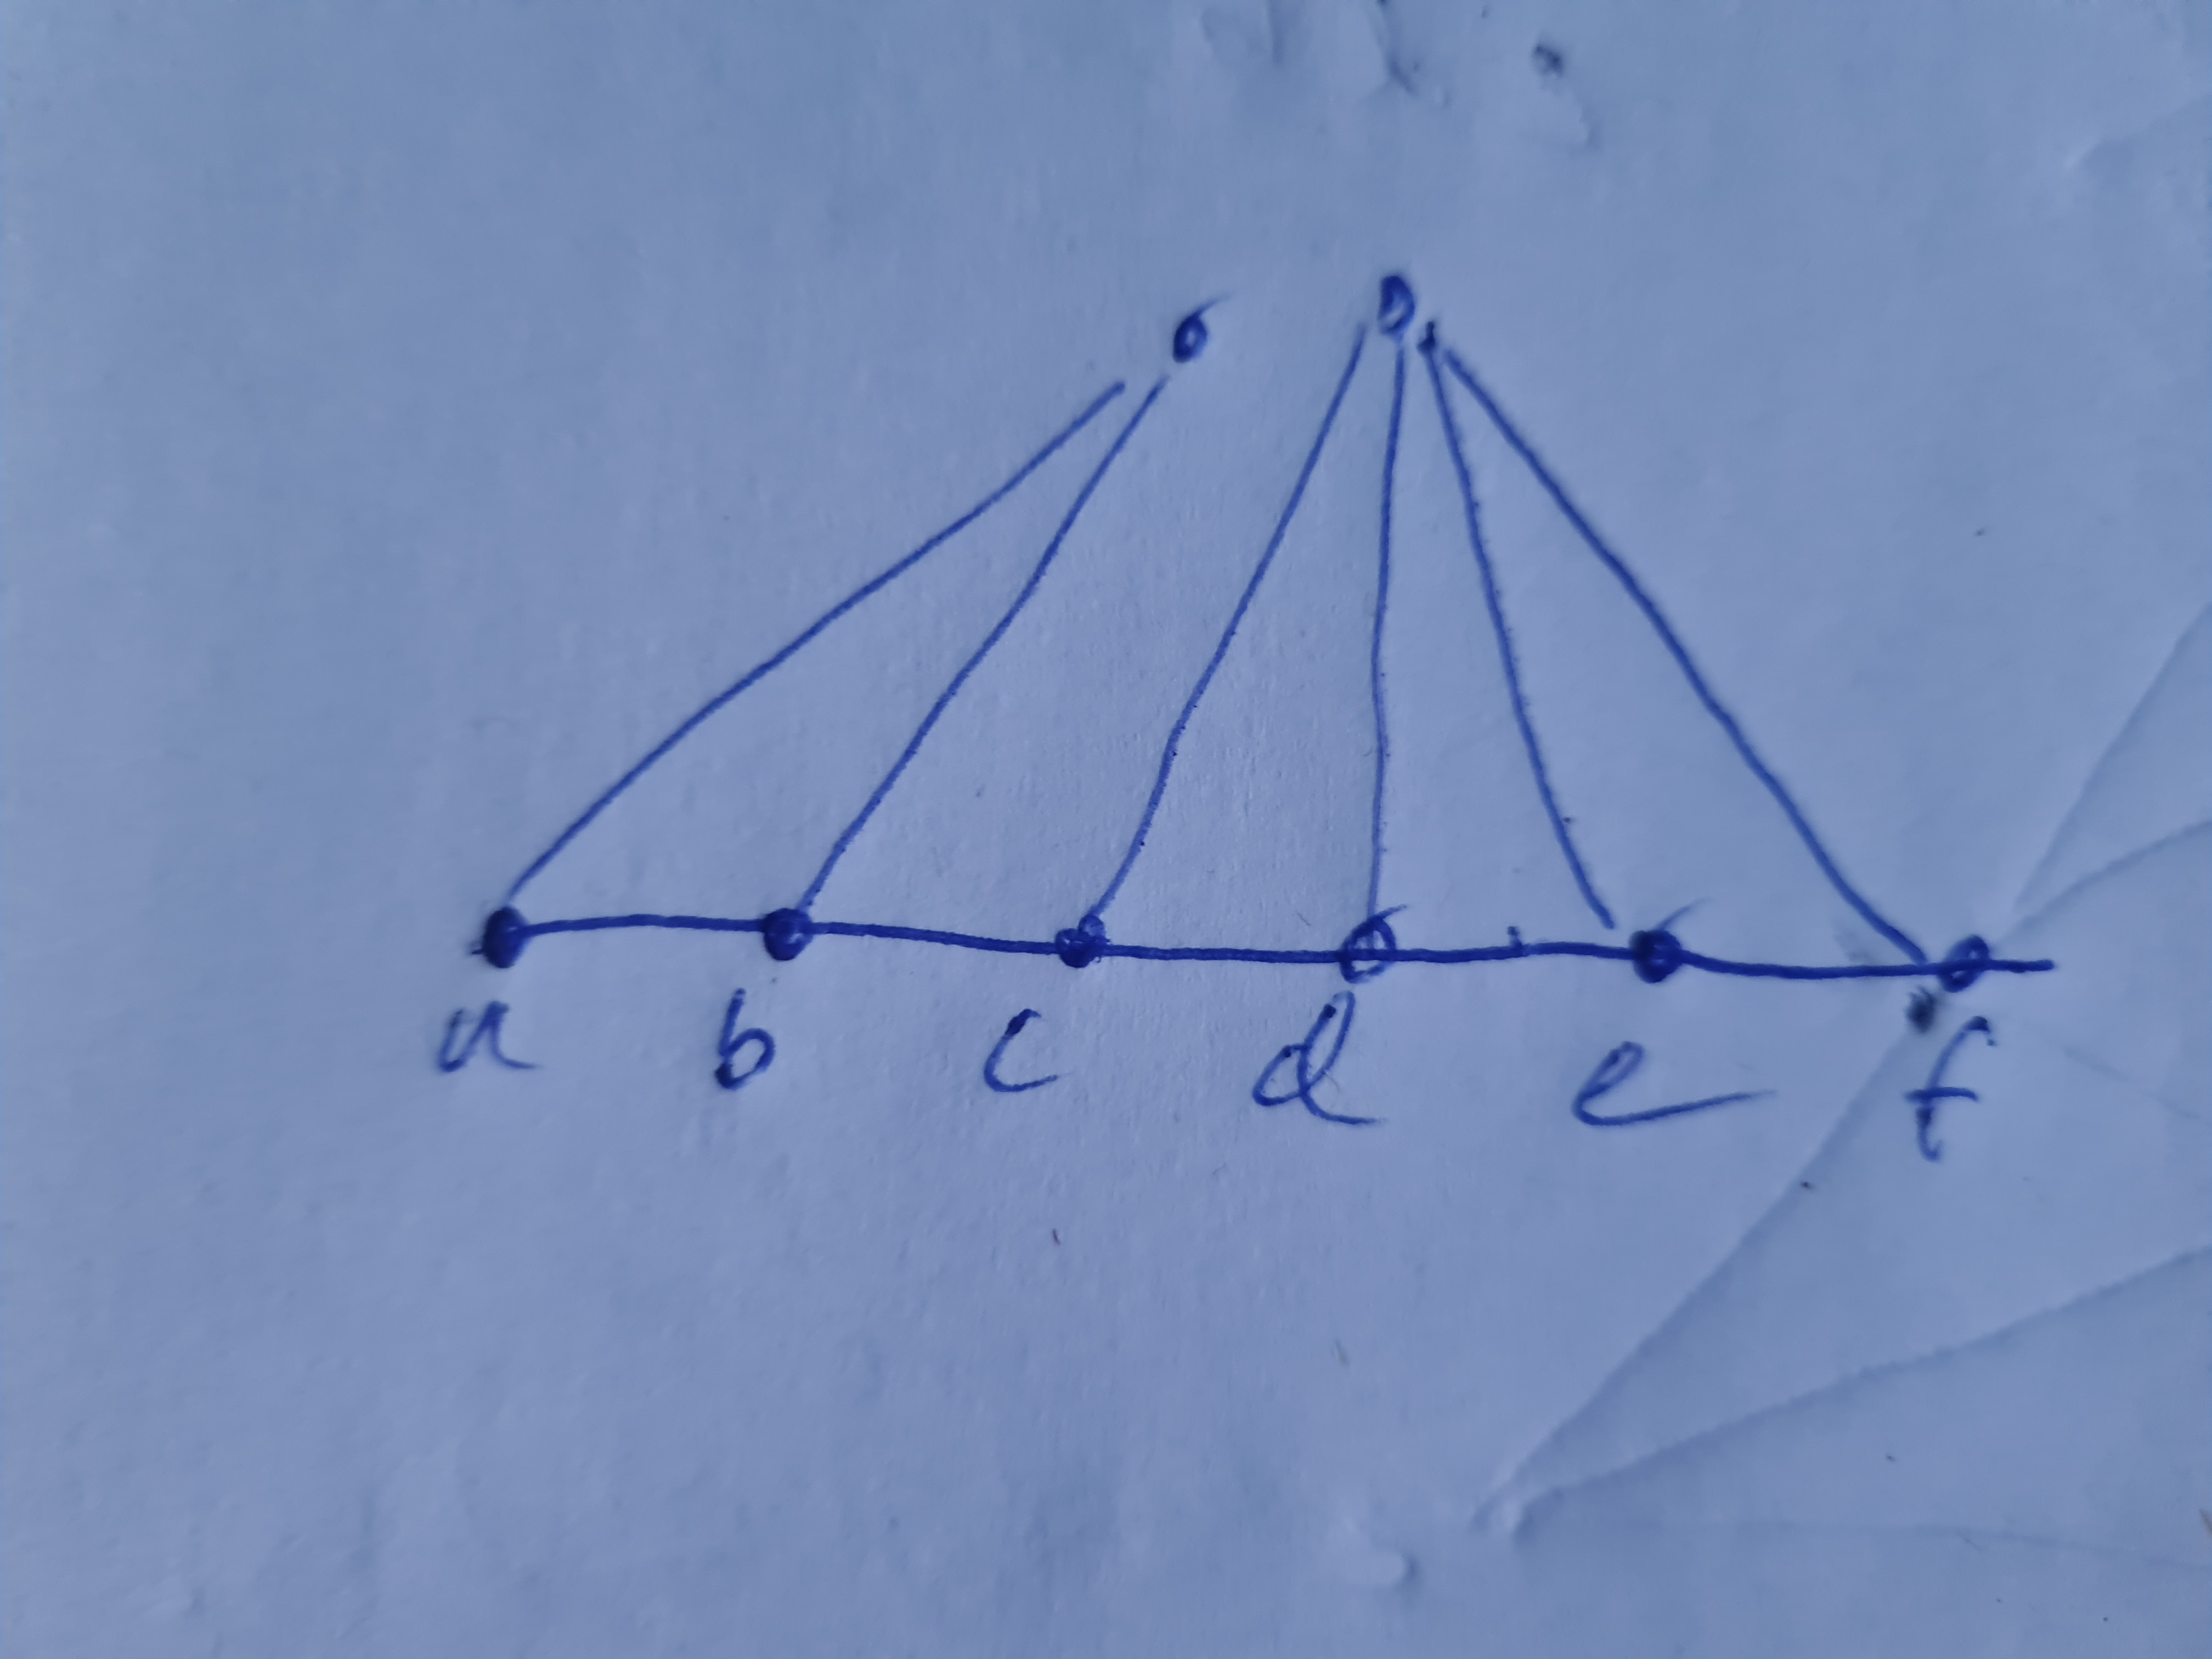
\includegraphics[width=0.5\textwidth]{q4a.jpg}
    \caption{An attempt to represent $M$ as a bipartite graph}
\end{figure} 

However, we need $c, e$ to form a basis, and so $e$ must also connect to vertex 1!
But then we have $e$ matching to 1, $f$ matching to 2, and therefore they are a matchable pair! But this is a contradiction, as in $M$, $\{e, f\}$ is not a basis.
Thus any way we try and describe $M$ as a transversal matrix we fail, and so $M$ is not transversal.

It remains to show $M^*$ is transversal.
Now our bases are of size 2, and so our cobases are of size 4. In particular, 
to find a basis of $M^*$ we simply choose 2 vertices that are not a parallel pair. Then, the remaining 4 vertices are connected.
In other words, a basis of $M^*$ is any basis of $M$, together with the remaining parallel pair!
So every basis of $M^*$ has one element from each parallel pair in $M^*$, and one additional element chosen from the remaining 3 vertices.
It is therefore simple to see how this creates a transversal representation.
\begin{figure}
    \label{representation}
    \centering
    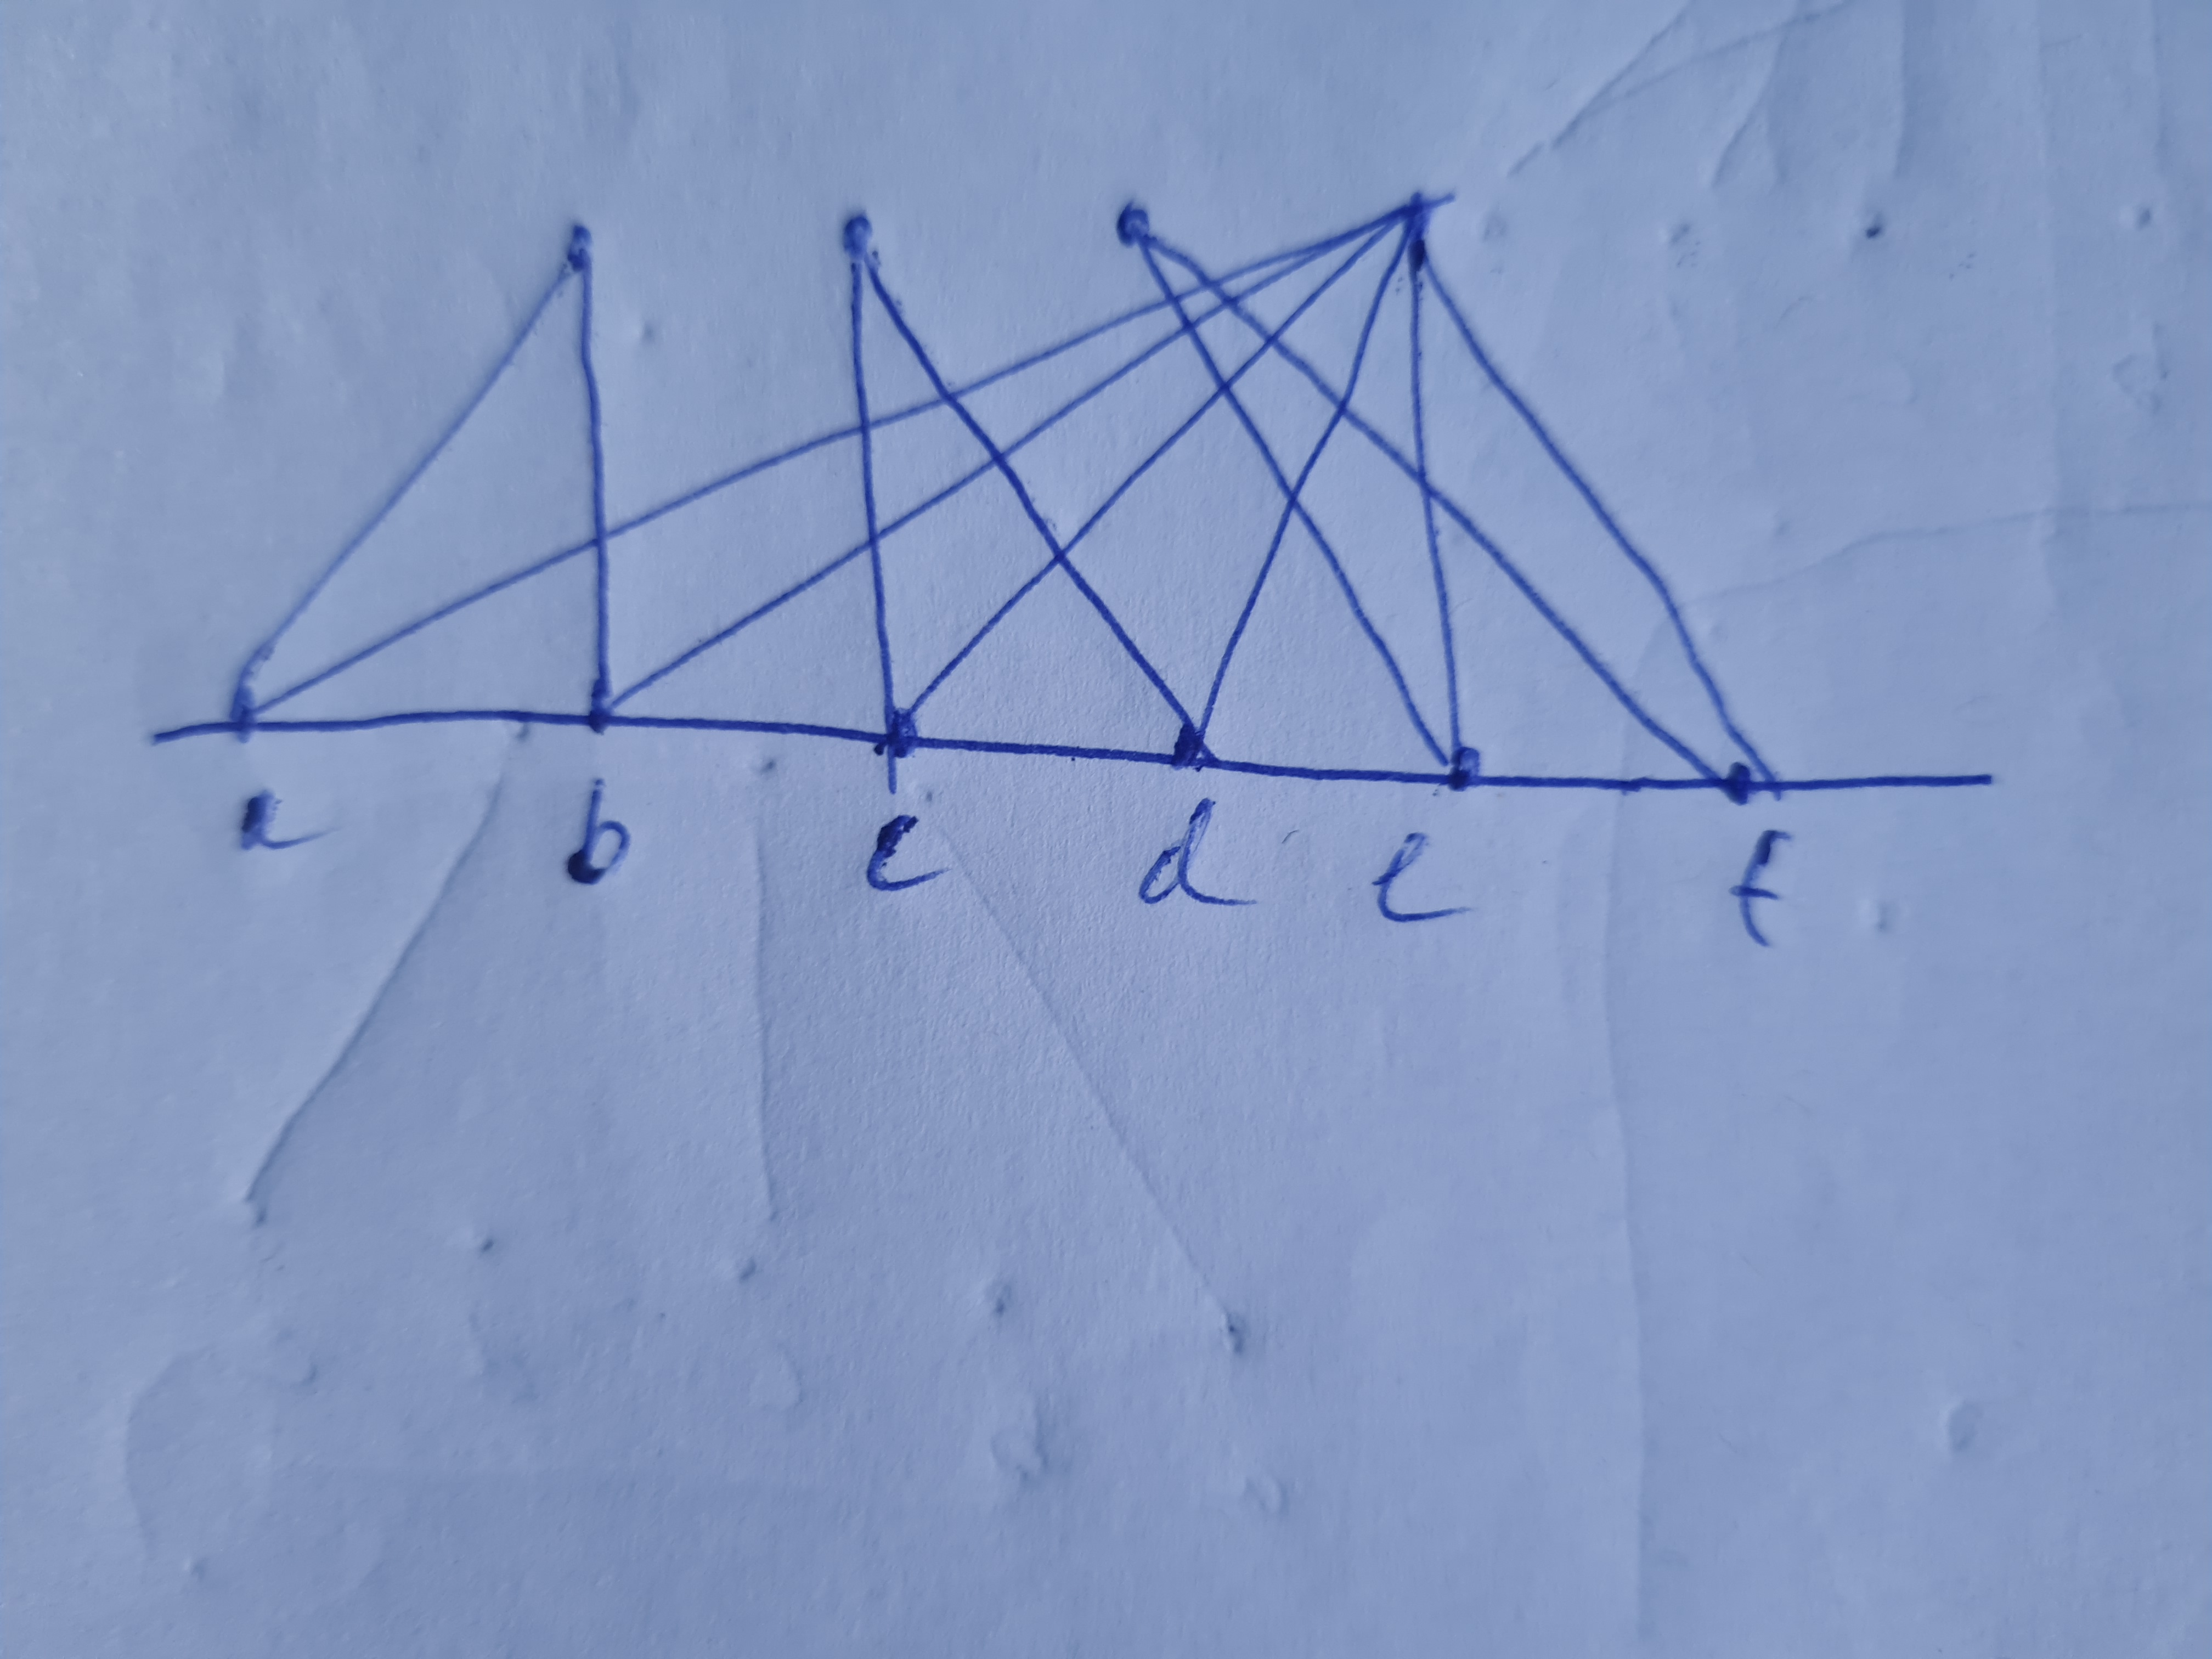
\includegraphics[width=0.5\textwidth]{q4c.jpg}
    \caption{A transversal representation of $M^*$, whose dual is not transversal}
\end{figure}
So to conclude, $M^*$ is transversal, but $(M^*)^*=M$ is not!


\section*{Question 5}
Firstly, we observe that $\{a, g, d, c\}$ form a hyperplane, and thus 
$\{b, f, e\}$ are colinear in $M^*$. However, 
we also have $\{b, e, d\}$, $\{b, f, a\}$, $\{c, e, f\}$ forming hyperplanes,
and therefore $\{g, d, c, e\}$, $\{g, f, c, a\}$, and $\{g, a, b, d\}$
are all coplanar. These are all the hyperplanes of $M$, and thus all the circuits of 
$M^*$. This gives us enough information to describe the matroid.
Firstly, note that these three planes must all intersect at $g$.
Apart from that, each plane pair shares exactly one other element,
and this is unique to each pair. Finally, each plane has exactly one unique element 
from our colinear triple.

So, the geometric representation should form some kind of trianglular pyramid 
at $g$, with each plane intersecting along a line, determined by the other element they share.
Finally, the remaining 3 elements, $\{b, e, f\}$, (one on each plane) are colinear,
so I draw a circle around them :).
\begin{figure}[!htb]
    \centering
    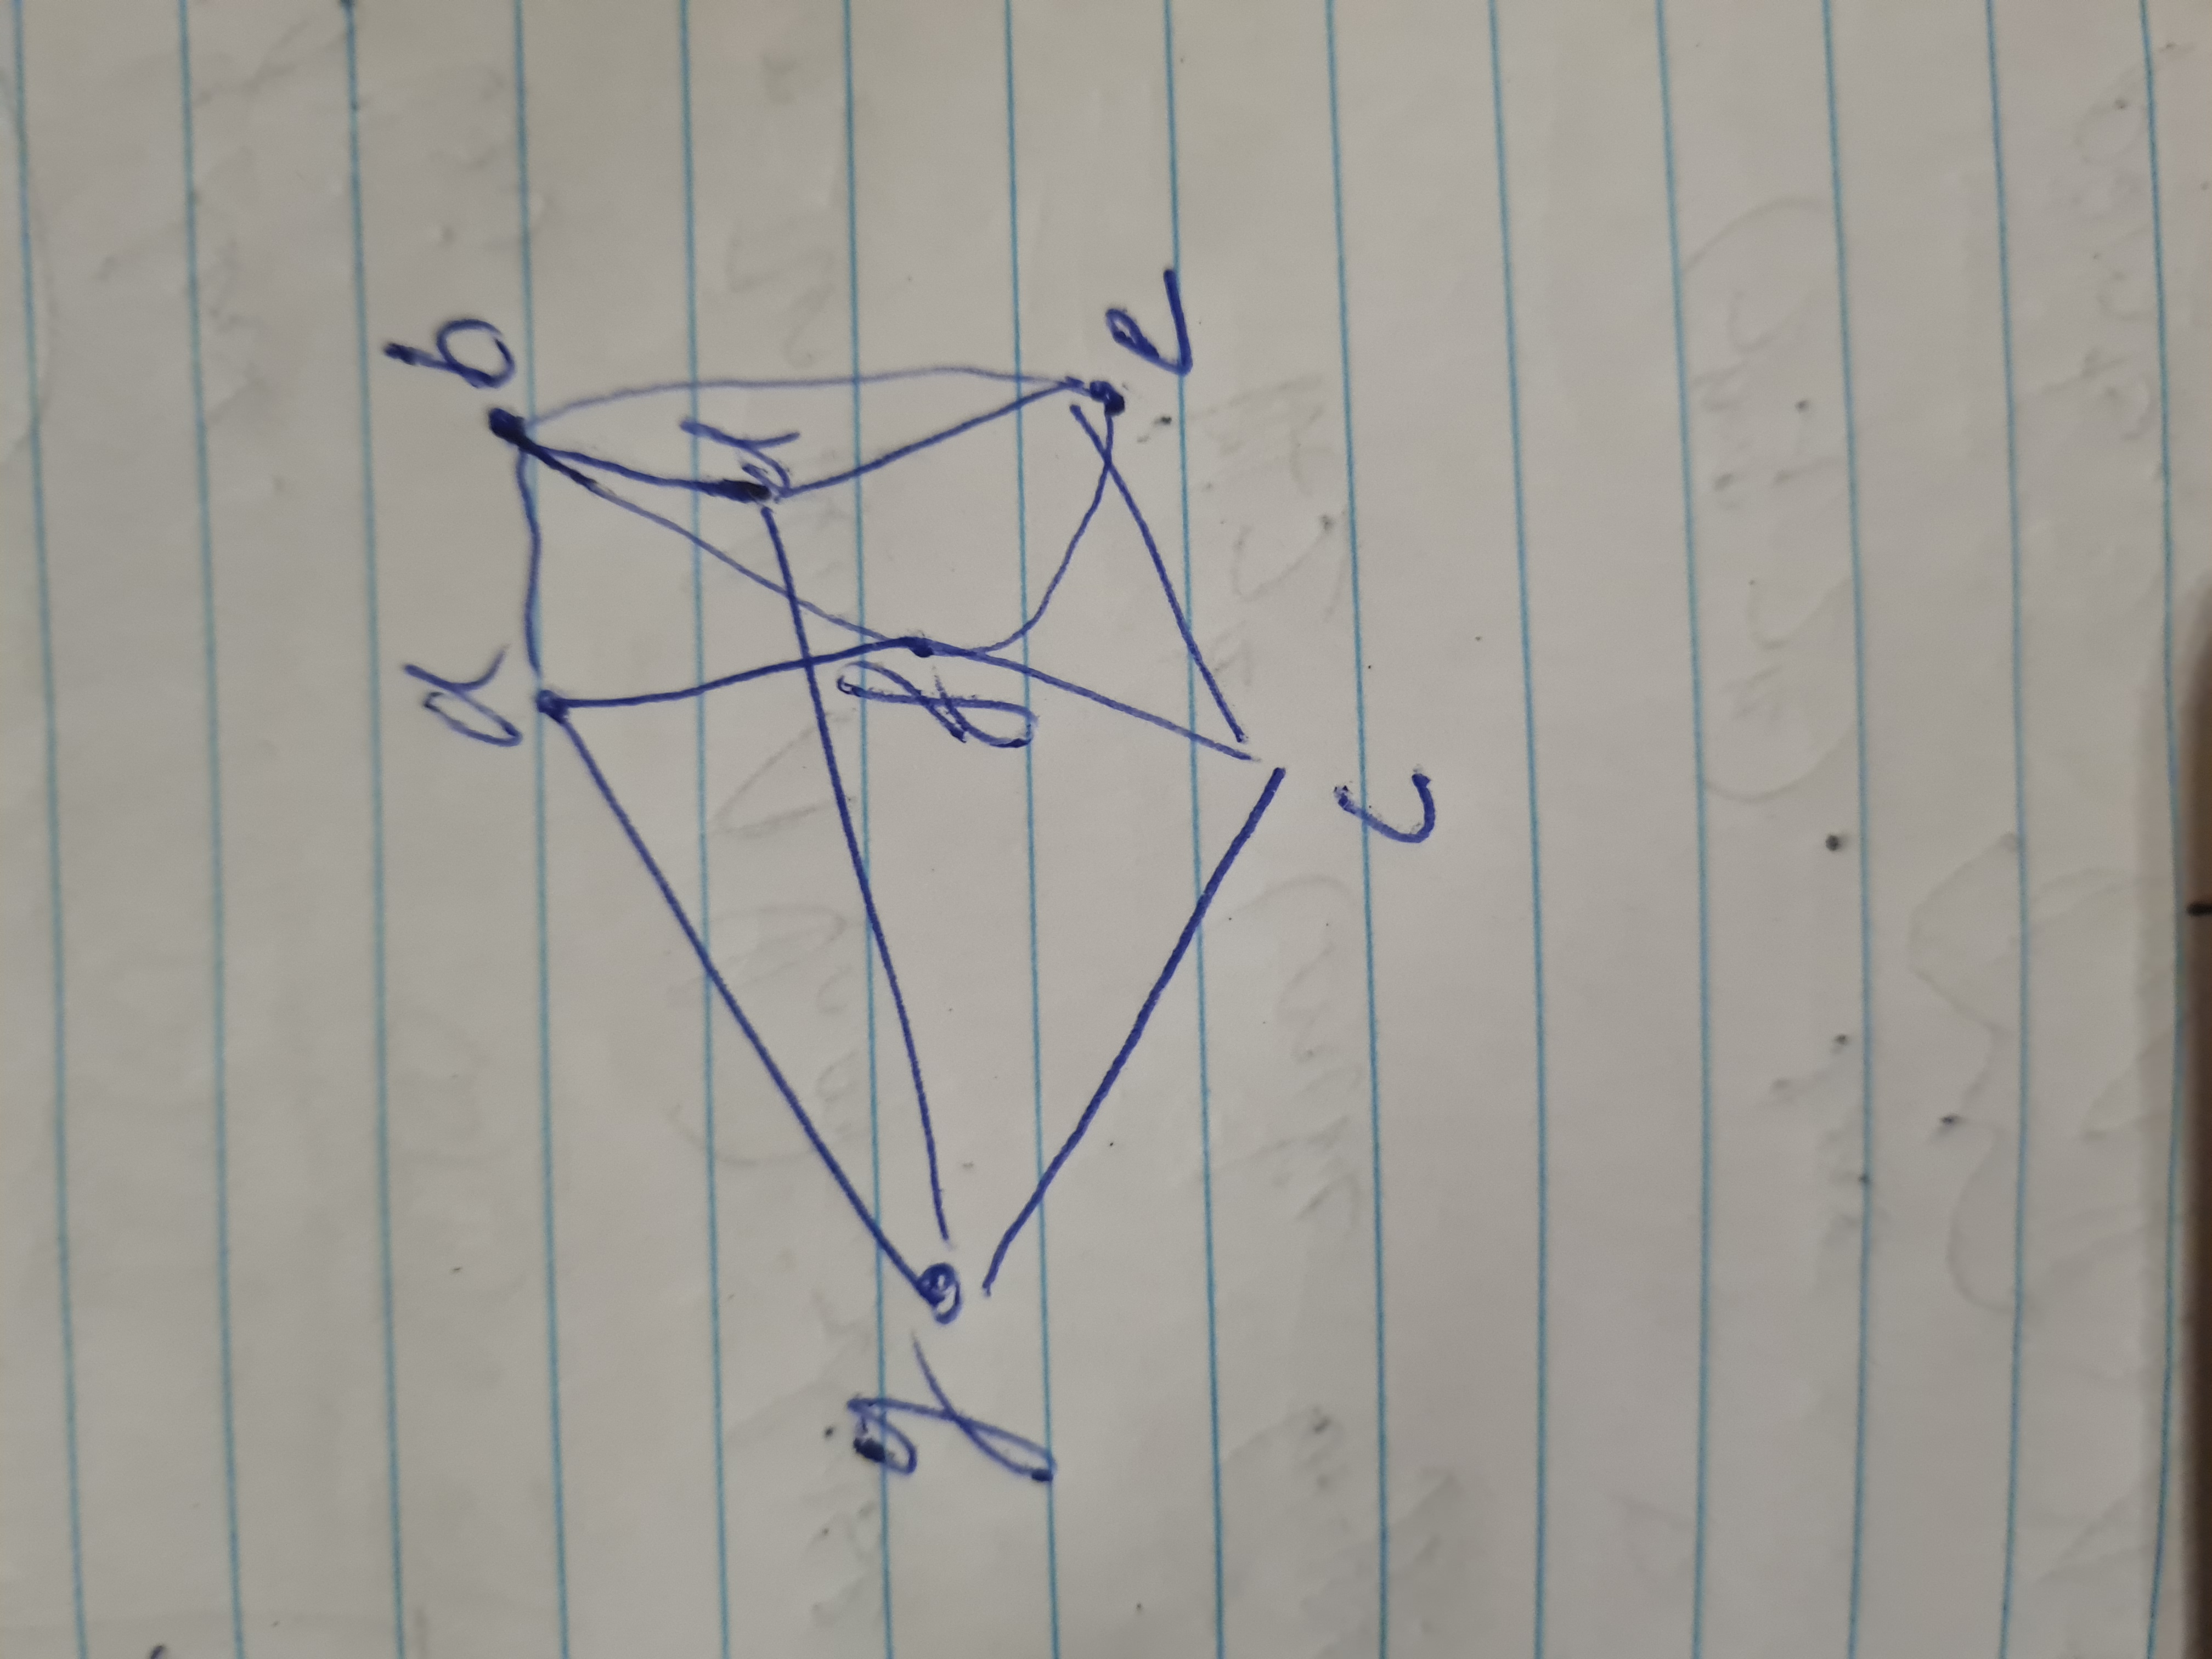
\includegraphics[width=0.5\textwidth, angle=-90]{q4.jpg}
    \caption{Question 5}
\end{figure}
\section*{Question 6}
Suppose $M=(E, \mathcal{B})$ is a self-dual matrix, ie $M=M^*$.
Let $B\subseteq \mathcal{B}$ be a basis in $M$. Then $E\backslash B\in \mathcal{B}(M^*)=\mathcal{B}$.
So both $B, E\backslash B$ are bases for $M$. But now, as seen in class all bases have the same size.
Additionally, we clearly have $B\cap (E\backslash B)=\emptyset$.
Thus, we have $|E|=|B\cup (E\backslash B)|=|B|+ |E\backslash B|=2|B|$, which is even.

\section*{Question 7}
\begin{enumerate}
    \item[i] Let $M$ be sparse paving with rank $r$, and suppose $C$ is a circuit of $M$ with size $r$.
        As seen in class, $X\subseteq E(M)$ is a hyperplane if $r(X)=r(M)-1$, and for any $e\not\in X$, $X\cup e$ is spanning.

        Firstly, we have that any subset of $C$ is independent, and $C$ itself is dependent. So $C$ contains an $r-1$ element 
        independent subset, but is not independent itself. Hence $r(C)=|C|-1=r(M)-1$.
        Now, take any $e\not\in C$. We will show $C\cup e$ contains a basis. Take $x\in C$, and consider $(C\backslash x)\cup e$.
        By assumption, $C\backslash x$ is independent. 
        Firstly, if $(C\backslash x)\cup e$ is independent, then as an independent set of size $r$, it is a basis contained in $C\cup e$
        and we are done.
        So assume towards a contradiction that it is dependent. 
        Removing any element of $(C\backslash x)\cup e$, we see that its size is less than $r(M)$,
        and so cannot be a circuit. Hence $(C\backslash x)\cup e$ is a circuit.
        But then, $C\cap ((C\backslash x)\cup e)=C\backslash x$. As seen above, this has size $r(M)-1$. 
        But that contradicts the fact that $M$ is sparse paving, and so $(C\backslash x)\cup e$ must be a basis for $M$.

        Hence $C\cup e$ is spanning, and thus $C$ is a hyperplane.

    \item[ii] 
        Recall the defintition of a sparse paving matrix from assingment 1:
        $M$ is sparse paving if $M\cong U_{0, n}$, $M\cong U_{n, n}$, or $M\cong(E, B_{r, C'})$ for some $n$ or $E, r, C'$.

        Firstly, note that $(U_{0, n})^*=U_{n, n}$, so this case follows trivially. 
        So suppose $M\cong(E, \mathcal{B}_{r, C'})$ for some $r, E$, and $C'$ a collection of $r$-element subsets of $E$
        (where $\mathcal{B}_{e, C'}$ is the collection of $r$ element subsets of $E$ not in $C'$).

        Now, consider $M^*=(E, \mathcal{B}^*)$, where $B^*=\{E\backslash B: B\in \mathcal{B}_{r, C'}\}$. Let $X$ be an $|E|-r$ element subset of $E$, not in $\mathcal{B}^*$.
        Now, we clearly have $X= X\backslash (E\backslash X)$. Now $|E\backslash X|=|E|-(|E|-r)=r$, and by assumption, it is not a basis.
        So $E\backslash X\in C'$. Conversely, for any $C\in C'$ we evidently have $E\backslash C\not\in \mathcal{B}^*$.
        Therefore $\{X\subseteq E: |X|=|E|-r, X\not\in \mathcal{B}^*\}=\{E\backslash C: C\in C'\}$. Call this set $C^{\prime *}$.

        So, the set of bases of $M^*$ are exactly the $|E|-r$ element subsets of $E$, not in $C^{\prime *}$.
        Thus $M^*\cong (E, \mathcal{B}_{|E|-r, C^{\prime *}})$, and thus it is sparse paving too.
\end{enumerate}
\end{document}


